\RequirePackage[l2tabu, orthodox]{nag}
\documentclass[12pt]{article}

\usepackage{amssymb,amsmath,verbatim,graphicx,microtype,upquote,units,booktabs,amsthm,listings,xcolor,tikz}
\usetikzlibrary{automata,positioning}

\newcommand{\problem}{
    \addtocounter{section}{1}
    \section*{Problem \#\thesection}
}
\newtheorem{theorem}{Theorem}

\lstset{language=C++,
                basicstyle=\footnotesize\ttfamily,
                keywordstyle=\color{blue}\ttfamily,
                stringstyle=\color{red}\ttfamily,
                commentstyle=\color{gray}\ttfamily,
                keepspaces=true,
                tabsize=2,
                breaklines=true
                }


\title{Quiz \#10}
\date{\today}
\author{Illya Starikov}

\begin{document}
\maketitle

\problem
\begin{align*}
    S& \\
    \implies AB &\quad\quad \text{via $S \rightarrow AB$} \\
    \implies aXB &\quad\quad \text{via $A \rightarrow aX$} \\
    \implies aXbYd &\quad\quad \text{via $B \rightarrow bYd$} \\
    \implies aXbYd &\quad\quad \text{via $B \rightarrow bYd$} \\
    \implies abXYd &\quad\quad \text{via $Xb \rightarrow bX$} \\
    \implies abYcd &\quad\quad \text{via $XY \rightarrow Yc$} \\
    \implies abcd &\quad\quad \text{via $Y \rightarrow \lambda$}
\end{align*}

\problem
\begin{align*}
    S& \\
    \implies TbC &\quad\quad \text{via $S \rightarrow TbC$} \\
    \implies gC &\quad\quad \text{via $Tb \rightarrow g$} \\
    \implies Sg &\quad\quad \text{via $gC \rightarrow Sg$} \\
    \implies TbCg &\quad\quad \text{via $S \rightarrow TbC$} \\
    \implies gCg &\quad\quad \text{via $Tb \rightarrow g$} \\
    \implies Sgg &\quad\quad \text{via $gC \rightarrow Sg$} \\
    \implies TbCgg &\quad\quad \text{via $S \rightarrow TbC$} \\
    \implies gCgg &\quad\quad \text{via $Tb \rightarrow g$} \\
    \implies egg &\quad\quad \text{via $gC \rightarrow e$}
\end{align*}


\problem
The language is derived by the grammar is $L = \{ aa a^n b^k \, | \, 0 \leq n \leq k,  n + k = 2c \} $, for some arbitrary constant $c$ (i.e. $n + k$ is even).

\problem
The following always halts, regardless of the input from $\Sigma = \{ 0, 1 \}$.

\begin{center}
    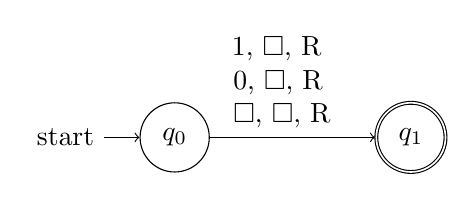
\begin{tikzpicture}[node distance=3cm,on grid,auto]
       \node[state,initial] (q_0)   {$q_0$};
       \node[state,accepting](q_1) [right=of q_0] {$q_1$};
       \path[->]
       (q_0) edge [text width=1.5cm] node {
       1, $\square$, R \\
       0, $\square$, R \\
       $\square$, $\square$, R
       } (q_1);
    \end{tikzpicture}
\end{center}

\problem
The following never halts, regardless of the input from $\Sigma = \{ 0, 1 \}$. Note it also never halts even if the tape is blank ($\lambda$).

\begin{center}
    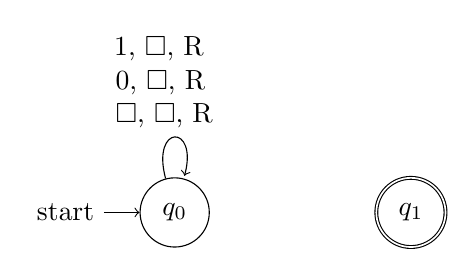
\begin{tikzpicture}[node distance=3cm,on grid,auto]
       \node[state,initial] (q_0)   {$q_0$};
       \node[state,accepting](q_1) [right=of q_0] {$q_1$};
       \path[->]
       (q_0) edge [loop above,text width=1.5cm] node {
       1, $\square$, R \\
       0, $\square$, R \\
       $\square$, $\square$, R
       } ();
    \end{tikzpicture}
\end{center}

\problem
The following halts for some, but not all, input from $\Sigma = \{ 0, 1 \}$. In this case, the only input that would cause the machine to halt would be $0$.
\begin{center}
    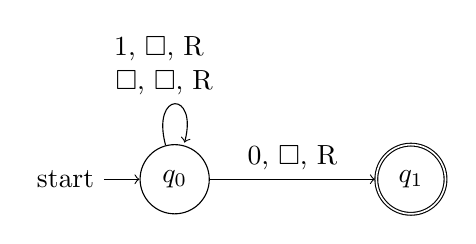
\begin{tikzpicture}[node distance=3cm,on grid,auto]
       \node[state,initial] (q_0)   {$q_0$};
       \node[state,accepting](q_1) [right=of q_0] {$q_1$};
       \path[->]
       (q_0) edge node {0, $\square$, R} (q_1)
             edge [loop above,text width=1.5cm] node {
       1, $\square$, R \\
       $\square$, $\square$, R
       } ();
    \end{tikzpicture}
\end{center}

\problem
No, we will prove so as follows.

\begin{theorem}
Suppose $A$ to be an arbitrary program --- that is, $A \in \text{all programs}$. Then, $\forall A \in \text{all program}$, there \textbf{does not} exists a program $P$ such that $P$ can determine if $A$ will halt \textbf{regardless of input}.
\end{theorem}

\begin{proof}
Suppose not. That is, suppose $\exists P \in \text{all programs}$ such that $P$ can determine if $\forall A \in \text{all programs}$, $A$ will halt. Suppose the following to be such program $P$, with an additional source code at the end:

\begin{lstlisting}[mathescape]
bool willHalt(program P) { $\cdots$ }

int recursiveNightmare() {
    if (willHalt(P)) {
        return recursiveNightmare();
    }

    return 42;
}

\end{lstlisting}

If we were to run this program through $P$, that is $P(P)$, we have the following cases:

\begin{description}
    \item [Case \#1:] The program $P$ loops forever. Assuming the program to be correct, this will return false; hence program $P$ halts on input $P$, which is a contradiction (by our \texttt{recursive nightmare}).
    \item [Case \#2:] The program halts on input $P$. Assuming the program to be correct, this will return true; hence program $P$ runs indefinitely on input $P$; this is a contradiction.
\end{description}

We see this to be a paradox; $P$ only halts when \texttt{willHalt} will not halt, and runs indecently when it does halt. Either way, we see this to be a contradiction. Therefore, there \textbf{does not} exists a program $P$ such that $P$ can determine if $A$ will halt \textbf{regardless of input}.

\end{proof}

\end{document}
